\documentclass{ethpresentation}
% \setbeameroption{show notes on second screen}

% Simple handout with just the slides
% "article" mode is better, but this might be useful in a pinch?
% \documentclass[handout]{ethpresentation}
% \usepackage{pgfpages}
% \pgfpagesuselayout{6 on 1}[a4paper,border shrink=5mm]

\title{Building a 25 MHz NMR Spectrometer}
\date{\today}
\author{Maximilian Stabel}
\institute{ETH Zürich}

\begin{document}
\maketitle % show when people are walking in

% Attention Getter
\begin{frame}{}
  \begin{center}
    \enquote{I have not yet lost that sense of wonder, and of delight, that this delicate motion should reside in all ordinary things around us, revealing itself only to him who looks for it.}

    \enquote{There the snow lay around my doorstep -- great heaps of protons quietly precessing in the Earth's magnetic field.}
  \end{center}

  \hfill{}--- E.M. Purcell
  \note[item]{I wouldn't have thought I would get a glimpse of this wonder Purcell describes when starting my thesis here, but I'm glad I did.}
  \note[item]{And I hope none of you have lost it yet}
  %\enquote{Most new insights come only after a superabundant accumulation of facts have removed the blindness which prevented us from seeing what later comes to be regarded as obvious. --- Isidor Isaac Rabi}
\end{frame}




\section{Why?}

\begin{frame}{Accessing NMR in the South is hard}
  \centering
  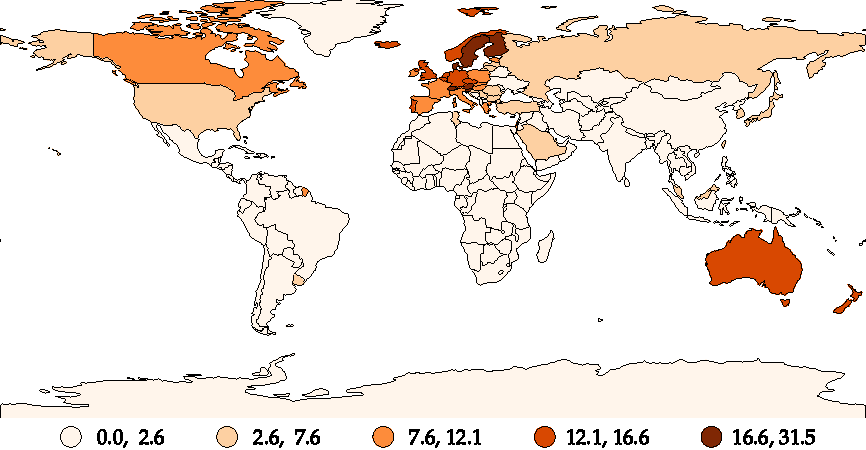
\includegraphics[height=0.8\textheight]{images/nmr-affiliations-per-million-people_naturalbreaks.pdf}

  \(\frac{\text{NMR affiliations}}{\text{million people}}\)
\end{frame}


\section{What does it look like?}

\section{What already works}

\begin{frame}{We can already see a water FID}
  \centering
  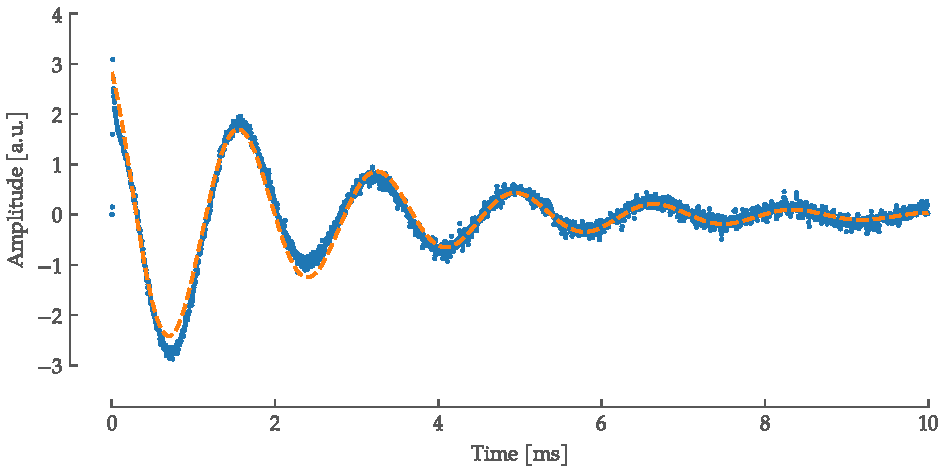
\includegraphics[width=0.9\textwidth]{images/fid_sine_fit.pdf}
\end{frame}

\begin{frame}{\ldots and do a Fourier transform}
  \centering
  \begin{tikzpicture}
    \node (fft)
    {
      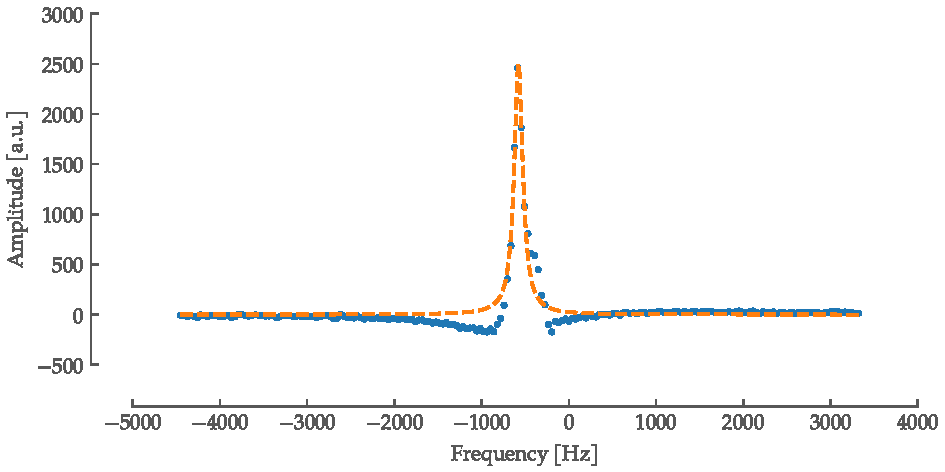
\includegraphics[width=0.9\textwidth]{images/fft_fit.pdf}
    };
    \begin{scope}[overlay]
      \node (structure) at (fft.north)
      [
        anchor=center,
        xshift=0.65cm,
        yshift=0cm
      ]
      {
        \includesvg[height=0.1\textheight]{images/h2o.svg}
      };
      \path[draw=grey,dashed,->] ([yshift=1mm,xshift=-3mm]structure.south east) to ([xshift=0.7cm,yshift=2.5cm]fft.center);
      \path[draw=grey,dashed,->] ([yshift=1mm,xshift=3mm]structure.south west) to ([xshift=0.6cm,yshift=2.5cm]fft.center);
    \end{scope}
  \end{tikzpicture}
\end{frame}

\begin{frame}{Toluene also has a visible signal}
  \centering
  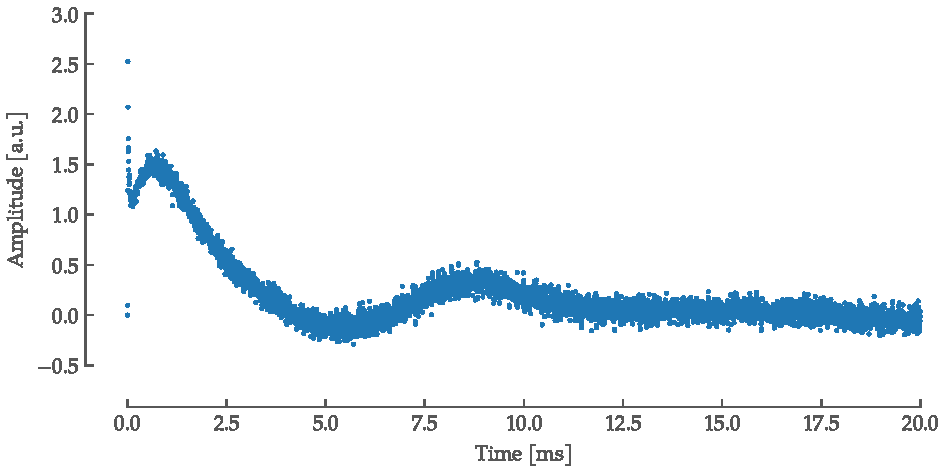
\includegraphics[width=0.9\textwidth]{images/fid_toluene.pdf}
\end{frame}

\begin{frame}{We can even see the Toluene peaks!}
  \centering
  \begin{tikzpicture}
    \node (fft)
    {
      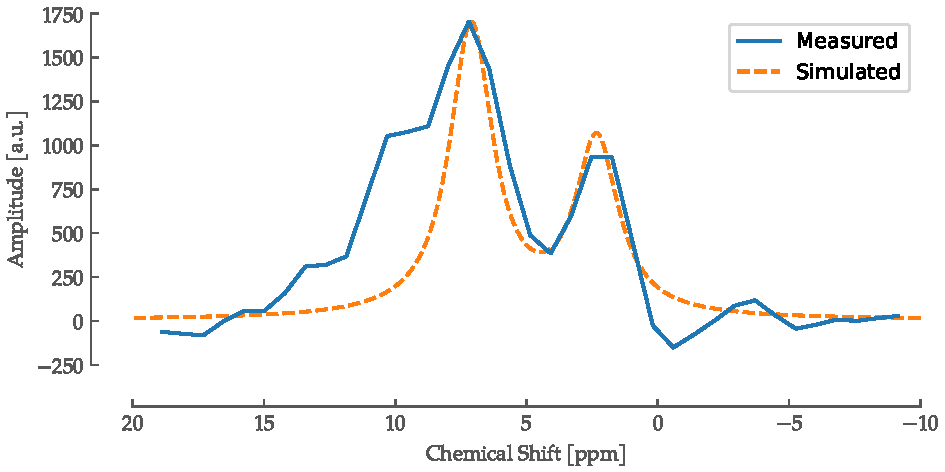
\includegraphics[width=0.9\textwidth]{images/fft_toluene.pdf}
    };
    \begin{scope}[overlay]
      \node (structure) at (fft.north)
      [
        anchor=north west,
        xshift=0mm,
        yshift=1.5cm
      ]
      {
        \includesvg[height=0.15\textheight]{images/toluene.svg}
      };
      \path[draw=grey,dashed,->] ([yshift=5mm,xshift=-4mm]structure.south east) to ([yshift=1.5cm,xshift=1.75cm]fft.center);
      \path[draw=grey,dashed,->] ([yshift=2mm,xshift=2mm]structure.south west) to ([yshift=2.75cm]fft.center);
    \end{scope}
  \end{tikzpicture}
\end{frame}

\begin{frame}{Thank you!}
  \begin{columns}
    \begin{column}{0.5\textwidth}
      \centering
      \includesvg[width=0.5\textwidth]{./images/logo_magnETHical.svg}
    \end{column}
    \begin{column}{0.5\textwidth}
      \centering
      Find everything on \\ \vspace*{\baselineskip}

      \includesvg[width=0.5\textwidth]{./images/gitlab_qrcode.svg}

      \url{https://gitlab.ethz.ch/mstabel/nmr-spectrometer}
    \end{column}
  \end{columns}
\end{frame}

\appendix

\begin{frame}[standout]
  A backup graph for explaining things.
\end{frame}

\end{document}